% !TEX root = ../ITGO.tex

%\subsection*{Three-bar truss design problem}

The three-bar truss design problem \cite{TB} consists in minimizing the volume of a statically loaded three-bar truss. There are two continuous design variables and three nonlinear inequality constraints, based on the stress on each of the truss members ($\sigma$), with $f(\bm{x}^*) = 263.895843$. Figure \ref{fig:TB} shows the schematic view of the problem. %The full problem statement follows:

%\vspace{-0.5cm}

%\begin{align*}
\textbf{Minimize:} & \\
& f(\bm{x}) = 2 \sqrt{2} x_1 + l x_2\\[0.5em]
\textbf{subject to:} &\\
& g_1(\bm{x}) = \frac{\sqrt{2} x_1 + x_2}{\sqrt{2} x_1^2 + 2 x_1 x_2} P - \sigma \leq 0 \\
& g_2(\bm{x}) = \frac{x_2}{\sqrt{2} x_1^2 + 2 x_1 x_2} P - \sigma \leq 0 \\
& g_3(\bm{x}) = \frac{1}{\sqrt{2} x_2 + x_1 x_2} P - \sigma \leq 0 \\[0.5em]
\textbf{where:} & \\
& l = 100cm, \quad P = 2 kN/cm^2, \quad \sigma = 2 kN/cm^2 \\[0.5em]
\textbf{with bounds:} & \\
& 0 \leq x_1, x_2 \leq 1
\end{align*}

\vspace{0.5cm}


\begin{figure}[h]
    \begin{center}
    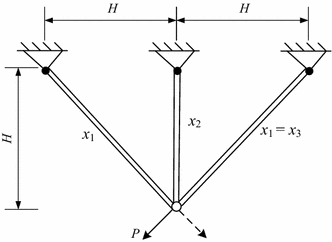
\includegraphics[scale=0.5]{img/Problems/TB.png}
    \end{center}
    \captionsetup{justification=centering}
    \caption{Schematic view of the three-bar truss design problem.}\label{fig:TB}
\end{figure}
